% !TEX root = ../main.tex

\chapter{排版图片}

\section{引言}
图应有自明性。插图应与文字紧密配合,文图相符,内容正确。选图要力求精练,插图、照
片应完整清晰。

\section{运动学分析}

考虑三个空间,分别是驱动空间、关节空间以及操作空间。驱动空间包含的是各个绳索长度组成的矩阵,不同时刻绳索长度可能不同。关节空间包含的是机械臂各个关节的关节角组成的矩阵,不同时刻关节角可能不同。操作空间包含的是机械臂末端位姿组成的位姿矩阵,不同时刻位姿可能不同,单个关节三维模型如\figref{fig:bm}所示。

\begin{figure}[ht]
\centering
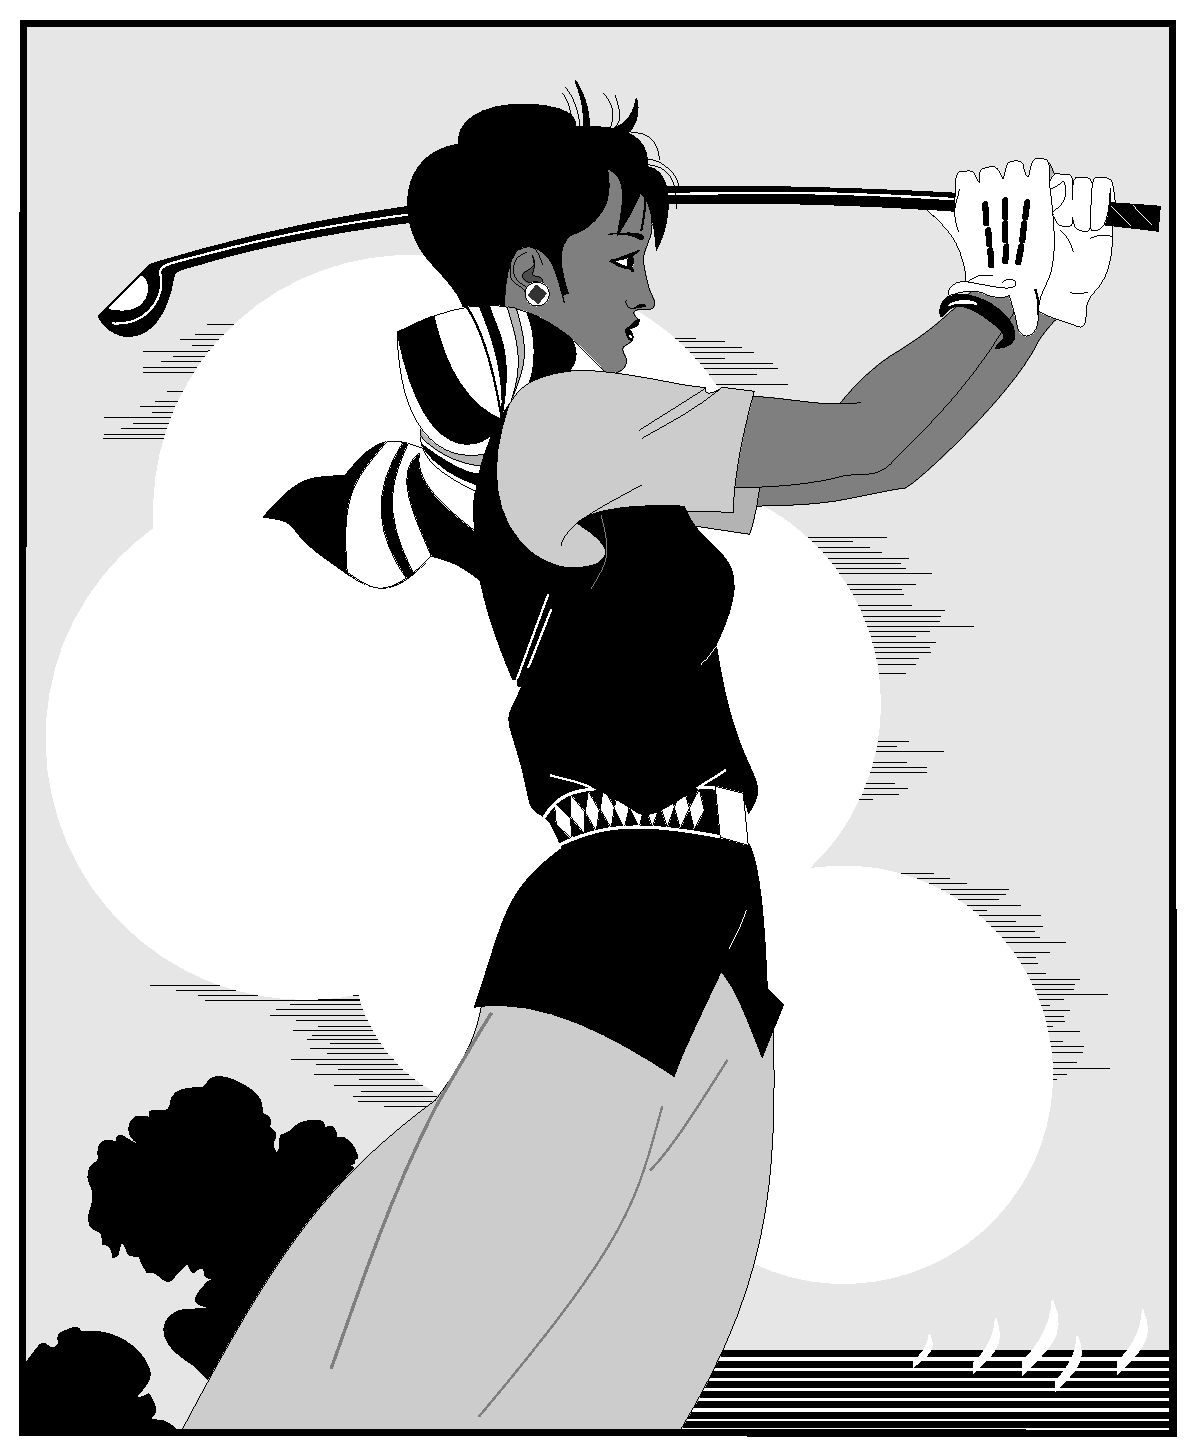
\includegraphics[width = 0.4\textwidth]{golfer}
\caption{打高尔夫球的人}
\label{fig:bm}
\end{figure}

\subsection{内容XXX}

\lipsum[3]

\section{内容XXX}

\lipsum[2]

\section{本章小结}

\lipsum[1]
